\chapter{Deep Learning Theory}
Notes based on blog by Desh Raj  \url{https://desh2608.github.io/}.

\section{Optimization}
Neural networks can be viewed as trying to minimize a loss function. The reason this is difficult is because the loss function is non-convex. Non-convex functions can have many local minima, saddle points, flat regions, and varying curvature which makes non-convex optimization at least NP-Hard (\url{https://www.cs.cornell.edu/courses/cs6787/2017fa/Lecture7.pdf}). If this is the case, why can deep networks find approximately reasonable solutions?

Almost all neural networks are trained by moving the parameters in the direction of a non-zero gradient. The goals of such descent are to find a critical point $\nabla =0$ and to find local optimum $\nabla =0$ and $\nabla^{2} >0$ (aka Hessian is positive semi-definite). 

\paragraph{Critical Points}
Parameter $\theta$, usually update in the following form: $\theta_{n+1} = \theta_{n} - \eta \nabla f(\theta_n)$. The hyper-parameter in the update equation is the learning rate, $\eta$. We know that we want it to be small but how do we know that $\eta$ is small enough? We utilize the Hessian aka $\nabla^2$. Suppose there exists some $\beta$ such that $-\beta I \leq \nabla^2 f(\theta) \leq \beta I$. Then a higher $\beta$ means $\nabla^2$ varies more so the learning rate should be lower. It can be more formally proved that in $O(\frac{\beta}{\epsilon^2})$, $\theta$ will arrive at a critical point.

\paragraph{Saddle Points}
One issue that such a descent may run into is the issue of saddle points. Several results (\url{http://proceedings.mlr.press/v40/Ge15.pdf}, \url{https://arxiv.org/pdf/1602.04915.pdf}, \url{https://arxiv.org/pdf/1703.00887.pdf}) show that gradient descent can be done by evading saddle points. The main ideas from these papers are that there are many saddle points but it is hard to converge to one and while Hessians can be used to avoid the saddle points, we do not actually have to because a noisy form of gradient descent converges to a local optimum in a polynomial number of steps. The last paper discusses how perturbed gradient descent does a better job of escaping saddle points than regular gradient descent. 

\section{Generalization}
What is impressive of most modern deep learning frameworks is that many generalize very well to test cases even when the number of parameters is greater than the number of training samples. This is counter-intuitive because one would think that deep neural networks would overfit with a small number of samples.

A common `folklore' experiment (discussed in \url{cs.princeton.edu/~rlivni/files/papers/LivnComputational.pdf}) 'is to show that for sufficiently over-specified networks, global optima are ubiquitous and in general computationally easy to find.' To understand this conceptually, think of fixing a 2 layer neural network with n hidden nodes. We provide it random inputs and collect the outputs. We then use these input/output pairs to train randomly initialized (2 layer) neural network. With only 2 layers, this would be quite difficult but it becomes easier when we increase the number of hidden nodes.

\paragraph{Capacity}
The capacity of a learning model can be viewed as the complexity of training samples that it can fit. A quadratic regression will have more capacity than linear regression. It can be proved that the following is true:\\

Test Loss - training loss $\leq \sqrt{\frac{N}{m}}$ where $N$ is the effective capacity and $m$ is the number of training samples. There are other measures such as Rademacher complexity and VC dimension that relate error to capacity. However, these fail for deep neural networks because the upper bounds from these measures are greater than 1. 

\paragraph{Excess Capacity}
\begin{figure}
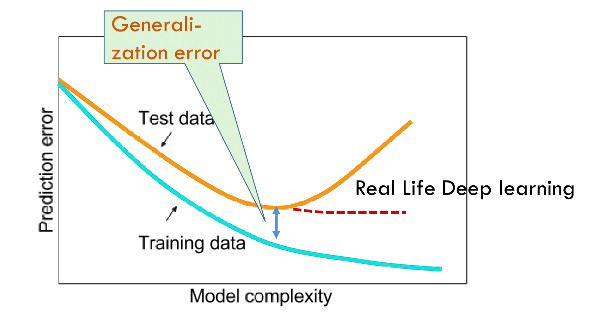
\includegraphics[width=1\textwidth]{capacity}
\end{figure}

From the figure we see that in general deep neural networks are able to generalize relatively well. For it was believed that the performance of deep neural networks did not necessarily mean high capacity and that a combination of stochastic gradient descent and regularization eliminates the excess capacity of a neural network. However, this was proved wrong in a paper from 2017 ( \url{https://arxiv.org/abs/1611.03530}). The experimental findings of the paper include that a classic convolutional neural net, like Alexnet, could be trained with random labels and still achieve high accuracy on training data. The paper proved that 'there exists a two-layer neural network with RELu activations and $2n+d$ weights that can represent any function on a sample size $n$ in $d$ dimensions. Recent work has shown that excess capacity can also exist in Kernel methods.

